\documentclass[conference]{IEEEtran}
\IEEEoverridecommandlockouts
\usepackage{cite}
\usepackage{amsmath,amssymb}
\usepackage{graphicx}
\usepackage{booktabs}
\usepackage{multirow}
\usepackage{xcolor}
\usepackage{url}
\graphicspath{{figures/}}
\newcommand{\ci}[2]{[$#1$,\,$#2$]}

\begin{document}

\title{Right for the Wrong Reasons? Auditing a Deep Brain-Age Model for Fairness, Acquisition Shortcuts and Explanation Faithfulness}

\author{
\IEEEauthorblockN{Adharshan N\IEEEauthorrefmark{1}\IEEEauthorrefmark{2}}
\IEEEauthorblockA{\textit{School of Computer Science and Engineering}\\
\textit{Vellore Institute of Technology}\\
Chennai, India\\
adharshan2706@gmail.com}
\and
\IEEEauthorblockN{Jaaiwanth K\IEEEauthorrefmark{1}\IEEEauthorrefmark{2}}
\IEEEauthorblockA{\textit{School of Computer Science and Engineering}\\
\textit{Vellore Institute of Technology}\\
Chennai, India\\
jaaiwanth90@gmail.com}
\and
\IEEEauthorblockN{Shridevi S\IEEEauthorrefmark{3}}
\IEEEauthorblockA{\textit{Centre for Neuroinformatics}\\
\textit{Vellore Institute of Technology}\\
Chennai, India\\
[faculty email]}
\thanks{\IEEEauthorrefmark{1}These authors contributed equally to this work.}
\thanks{\IEEEauthorrefmark{2}School of Computer Science and Engineering (SCOPE). \IEEEauthorrefmark{3}Corresponding author.}
}

\maketitle

\begin{abstract}
Brain-age models predict chronological age from structural MRI, and the brain-age gap (predicted minus chronological age) is widely studied as a marker of brain health. Such models are usually judged by accuracy alone, yet an accurate model can still be biased against subgroups or rely on non-anatomical shortcuts. We present a layered audit of a state-of-the-art brain-age network beyond accuracy. We fine-tuned the UK Biobank-pretrained Simple Fully Convolutional Network (SFCN) on 485 T1-weighted scans from the public IXI dataset (three London acquisition sites, ages 20--86). On a test set evaluated once, it reached a mean absolute error of 3.71 years (95\% CI 3.10--4.38; $r=0.966$) with no detectable sex disparity. However, scans from one site received an age-adjusted brain-age gap 5.06 years lower than the reference site (CI $-8.66$ to $-1.34$), an offset that replicated in an independent validation split. Three experiments show that the model is partly right for the wrong reasons: the acquisition site is decodable from its 64-dimensional representation with 91.2\% balanced accuracy after removing age and sex (chance 33\%); changing only a scan's intensity appearance to another site's shifts predicted age by 3--4 years in the same direction for every subject; and the offset is not explained by global intensity, matched image smoothness or the representation's site signature, which ComBat removes (probe 36.3\%) while leaving most of the offset. Attribution maps passed randomisation and deletion tests, and predictive uncertainty doubled on an unseen site while keeping 92\% coverage. We summarise the audit as a one-page model fairness passport and release all code.
\end{abstract}

\begin{IEEEkeywords}
brain age, MRI, fairness, shortcut learning, explainable AI, site effects, harmonisation, uncertainty
\end{IEEEkeywords}

%=====================================================================
\section{Introduction}
%=====================================================================
Brain-age models learn to predict a person's chronological age from a structural MRI scan \cite{cole2017trends,franke2019ten}. Applied to a new person, the brain-age gap (BAG) between predicted and chronological age is interpreted as accelerated or delayed brain ageing, and it has been associated with mortality, cognitive decline and neurological disease \cite{cole2018mortality}. Deep convolutional networks now predict age with errors of a few years \cite{cole2017deep,peng2021sfcn,bashyam2020dbn}.

Accuracy alone does not make a model trustworthy. First, a model can be accurate on average and still be systematically biased for a subgroup \cite{larrazabal2020gender,seyyed2021underdiagnosis,riccilara2022fairness}. For brain age, a subgroup bias means that the brains of one group look ``older'' or ``younger'' for reasons unrelated to biology \cite{picarra2023brainage}. Second, a model can be \emph{right for the wrong reasons}: deep networks exploit shortcuts \cite{geirhos2020shortcut}, and medical-imaging models are known to use hospital-specific acquisition properties instead of pathology \cite{zech2018pneumonia,degrave2021covid}. In multi-site MRI, scanner and protocol differences are a well-known source of such site effects \cite{glocker2019scanner,fortin2018harmonization,dinsdale2021unlearning}. Third, the explanations used to inspect a model can themselves be unfaithful \cite{adebayo2018sanity,hooker2019benchmark}.

This work audits a widely used brain-age network on the public IXI dataset along all three axes. We ask:
\begin{enumerate}
\item \textbf{Accuracy:} how accurate is a pretrained brain-age CNN on IXI, and what does fine-tuning add?
\item \textbf{Fairness:} once age is controlled for, do the error or the BAG differ by sex or by acquisition site, and does the model generalise to a site it never saw?
\item \textbf{Right for the wrong reasons?} Does the model's representation encode the acquisition site, does its prediction respond to acquisition appearance when anatomy is fixed, and can the site disparity be explained by measurable acquisition properties?
\end{enumerate}

Our contributions are:
\begin{itemize}
\item A reproducible, layered audit protocol for brain-age models that goes beyond accuracy (Fig.~\ref{fig:overview}), with age-adjusted group comparisons, bootstrap confidence intervals and a single use of the test set.
\item Evidence that a fine-tuned SFCN encodes the acquisition site (91.2\% probe accuracy) and that its predictions shift by 3--4 years under an \emph{age- and sex-standardised} acquisition-appearance swap that leaves anatomy unchanged.
\item A rule-out analysis showing that a robust 5-year site offset is \emph{not} explained by intensity profile, matched image smoothness or the representation's site signature, cautioning against attributing site disparities to ``scanner bias'' without testing.
\item Validation of the explanations and uncertainty used in the audit: attribution maps that pass randomisation and deletion tests, and predictive uncertainty that flags an unseen site while keeping near-nominal coverage.
\item A one-page \emph{model fairness passport} that turns the audit into actionable usage guidance, in the spirit of model cards \cite{mitchell2019modelcards}.
\end{itemize}

\begin{figure*}[t]
\centering
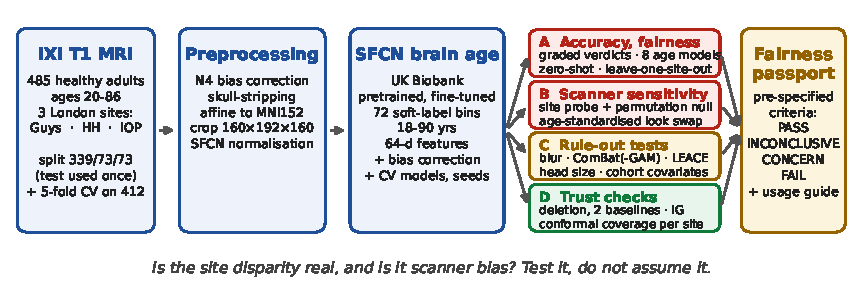
\includegraphics[width=\textwidth]{fig1_overview.pdf}
\caption{Overview of the audit. A UK Biobank-pretrained SFCN is fine-tuned on IXI and frozen; four audit layers (accuracy, group fairness, shortcut tests, trust checks) are then applied to held-out subjects only, and summarised as a fairness passport.}
\label{fig:overview}
\end{figure*}

%=====================================================================
\section{Related Work}
%=====================================================================
\textbf{Brain-age prediction.} Early brain-age models used regression on regional features \cite{franke2019ten}. Deep 3D CNNs trained on raw images \cite{cole2017deep}, DeepBrainNet trained on 14,468 individuals \cite{bashyam2020dbn} and the lightweight SFCN trained on UK Biobank \cite{peng2021sfcn} brought errors down to a few years. Brain-age estimates regress towards the mean age, so a linear bias correction is standard \cite{le2018nonlinear,smith2019delta,delange2020correction}.

\textbf{Fairness in medical imaging.} Imbalanced training data produces biased classifiers \cite{larrazabal2020gender}, and chest X-ray models underdiagnose under-served groups \cite{seyyed2021underdiagnosis}; see \cite{riccilara2022fairness} for a review. For brain age, Pi\c{c}arra and Glocker analysed race and sex bias in UK Biobank \cite{picarra2023brainage}. Group differences in performance are distinct from group information being \emph{encoded}: models encode protected characteristics even when not trained to \cite{glocker2023encoding}, which can be measured with linear probes \cite{alain2016probes}.

\textbf{Site effects and harmonisation.} Multi-site imaging carries scanner signatures that models can learn \cite{glocker2019scanner}. ComBat \cite{johnson2007combat} removes additive and multiplicative site effects and is widely used for MRI-derived measures \cite{fortin2018harmonization}; adversarial unlearning removes site information during training \cite{ganin2016dann,dinsdale2021unlearning}. Intensity standardisation by histogram matching is a classical MRI technique \cite{nyul2000standardization}.

\textbf{Faithful explanations and uncertainty.} Grad-CAM \cite{selvaraju2017gradcam} is the most common saliency method for CNNs, and HiResCAM provides faithful location-wise maps \cite{draelos2020hirescam}. Saliency maps should pass randomisation sanity checks \cite{adebayo2018sanity} and perturbation (deletion) tests \cite{samek2017evaluating,hooker2019benchmark}. Neural network confidence is often miscalibrated \cite{guo2017calibration}, so coverage of predictive ranges must be checked.

Prior brain-age studies typically report accuracy, sometimes group errors, and rarely test whether a disparity is caused by acquisition. Our audit combines these strands on a single frozen model and tests the shortcut hypothesis directly.

%=====================================================================
\section{Data}
%=====================================================================
\textbf{Dataset.} IXI \cite{ixi} provides T1-weighted MRI and demographics for healthy adults scanned at three London sites: Guy's Hospital (Guys; Philips 1.5\,T), Hammersmith Hospital (HH; Philips 3\,T) and the Institute of Psychiatry (IOP; GE 1.5\,T).

\textbf{Label correction.} An early version of our demographics table attached age and sex to the wrong subjects, because a row index had been used as the subject identifier. We rebuilt all labels from the official spreadsheet, joined on the IXI identifier. Two independent rebuilds by different team members agreed with the corrected labels. All results use the corrected labels.

\textbf{Exclusions and splits.} We excluded 14 scans (10 without a demographic record, 2 without age, 2 with conflicting duplicates). The remaining 485 subjects were split 339/73/73 into train, validation and test sets, stratified by site (Table~\ref{tab:data}). The test set (Guys 42, HH 22, IOP 9; 43 female, 30 male) was evaluated \emph{once}, after all modelling decisions had been made on train and validation data. IOP recruited younger participants, which is one reason every comparison below adjusts for age.

\begin{table}[t]
\caption{Subjects per acquisition site}
\label{tab:data}
\centering
\begin{tabular}{lcccc}
\toprule
Site & Scanner & Train $n$ & Train mean age & Held-out $n$ \\
\midrule
Guys & Philips 1.5\,T & 192 & 48.4 & 83 \\
HH   & Philips 3\,T   & 104 & 47.3 & 45 \\
IOP  & GE 1.5\,T      & 43  & 40.6 & 18 \\
\bottomrule
\multicolumn{5}{l}{\footnotesize Held-out = validation + test (146 subjects).}
\end{tabular}
\end{table}

%=====================================================================
\section{Methods}
%=====================================================================
\subsection{Preprocessing}
Each scan underwent N4 bias-field correction \cite{tustison2010n4}, skull-stripping in native space with ANTsPyNet \cite{tustison2021antsx}, brain-to-brain affine registration to the MNI152NLin6Asym 1\,mm template from TemplateFlow \cite{ciric2022templateflow}, and a centre crop to SFCN's $160\times192\times160$ input. Quality control used Dice overlap with the template brain, centre offset, edge truncation and native brain volume. Following SFCN's reference implementation, each volume is divided by its mean over the full $182\times218\times182$ template box; normalising by the mean of the cropped volume instead makes inputs about $1.47\times$ too small and collapses the pretrained model's outputs.

\subsection{Model and fine-tuning}
SFCN \cite{peng2021sfcn} is a 3D CNN with five convolution--batch-norm--max-pool--ReLU blocks and a $1\times1\times1$ block, followed by global average pooling to a 64-dimensional feature vector and a $1\times1\times1$ convolution that outputs a probability $p_k$ for each one-year age bin with centre $c_k$. The prediction is the expected value $\hat{y}=\sum_k p_k c_k$. The published UK Biobank head covers ages 42--82, so we replaced it with 72 bins covering 18--90, warm-starting the bins for 42--82 from the pretrained head. Training used Gaussian soft labels ($\sigma=2$ years) and a Kullback--Leibler loss, in two stages: the head only (5 epochs, learning rate $10^{-3}$), then the whole network with AdamW \cite{loshchilov2019adamw} (head $10^{-3}$, backbone $10^{-4}$) for up to 60 epochs with early stopping on validation MAE (patience 15) and learning-rate reduction on plateau. The selected checkpoint (epoch 30) was frozen for every analysis that follows.

As a replication, SFCN and DeepBrainNet \cite{bashyam2020dbn} were also fine-tuned independently with an alternative preprocessing pipeline on the same split.

\subsection{Evaluation and bias correction}
Following \cite{cole2018mortality,delange2020correction}, we fitted $\hat{y}=a\,y+b$ on the \emph{validation} set ($a=0.832$, $b=8.30$) and corrected predictions as $(\hat{y}-b)/a$. The corrected BAG is the corrected prediction minus chronological age. We report MAE, RMSE and Pearson $r$ with 95\% percentile-bootstrap CIs (5,000 resamples) \cite{efron1993bootstrap}.

\subsection{Fairness audit}
On the test set we fitted ordinary least-squares models $\mathrm{BAG}\sim\mathrm{sex}+\mathrm{site}+\mathrm{age}$ and $|\mathrm{error}|\sim\mathrm{sex}+\mathrm{site}+\mathrm{age}$ with HC3 robust standard errors \cite{mackinnon1985hc}, reference levels female and Guys, and bootstrap CIs. For \emph{leave-one-site-out} (LOSO) generalisation, three further models were each trained without one site and evaluated on that site's train and validation subjects (never the test set), against seen-site validation subjects.

\subsection{Attribution maps and their validity}
Standard Grad-CAM \cite{selvaraju2017gradcam} produced empty maps for 20--80\% of subjects at SFCN's layers, so we used the location-wise gradient $\times$ activation summed over channels (magnitude), a HiResCAM-style map \cite{draelos2020hirescam}, at block \texttt{conv\_2} ($20\times24\times20$ cells of 8\,mm), with the predicted age as target. This choice was made before any group comparison. Maps were upsampled, masked, normalised to unit sum and summarised as the share of attribution in 59 Harvard--Oxford regions grouped into 7 coarse regions \cite{jenkinson2012fsl}; group differences on held-out subjects ($n=146$) used $\mathrm{share}\sim\mathrm{sex}+\mathrm{site}+\mathrm{age}$ with Benjamini--Hochberg FDR \cite{benjamini1995fdr}.

We tested validity in two ways: a \emph{cascading randomisation} sanity check \cite{adebayo2018sanity}, re-initialising the layers above the target and comparing maps; and a \emph{deletion test} \cite{samek2017evaluating,hooker2019benchmark} on 60 held-out subjects, replacing the top-, bottom- or randomly-ranked 5/10/20\% of brain cells with a heavily smoothed copy of the image (Gaussian $\sigma=8$ voxels) and measuring $|\Delta\hat{y}|$. Smoothing keeps local intensity while removing anatomical detail, so every condition applies the same kind of perturbation and only its location differs.

\subsection{Shortcut tests}
All use the frozen model and held-out subjects; nothing is tuned on test labels.

\textbf{Site probe.} A class-balanced multinomial logistic regression (regularisation by 5-fold CV on train) was trained on the train subjects' 64-d pooled features to predict site, and scored on held-out subjects with balanced accuracy \cite{alain2016probes,glocker2023encoding}. We compared demographics only, input-intensity quantiles, pretrained and fine-tuned SFCN features, each with and without age, age$^2$ and sex regressed out.

\textbf{Acquisition stress test.} Each held-out brain's intensity distribution was quantile-matched (101 quantiles) \cite{nyul2000standardization} to each site's reference and its age predicted again. Because IOP recruited younger people and tissue proportions change with age, the references were built from train subjects and \emph{standardised to a common age and sex mix}: per site, the quantile vector was regressed on age, age$^2$ and sex and evaluated at the pooled train mean. Effects are expressed relative to matching to the subject's \emph{own} site, so the matching operation itself is controlled for. On 40 subjects we also varied single properties: contrast ($\gamma$), noise, Gaussian blur and smooth intensity non-uniformity.

\textbf{Image sharpness and matched blur.} We read native voxel sizes from the headers and computed three sharpness measures on the model input (mean gradient magnitude, Laplacian spread and a smoothness FWHM estimate \cite{forman1995fwhm}), compared across sites adjusting for age and sex. Each held-out Guys and HH brain was then blurred by exactly the amount that raises its FWHM to IOP's adjusted level, and re-predicted.

\textbf{Feature harmonisation.} The 64-d features were harmonised with ComBat (location/scale) \cite{johnson2007combat,fortin2018harmonization}, preserving age, age$^2$ and sex, with parameters estimated on train only. Age was re-predicted through the model's unchanged head; applying the head to the original features reproduces the model's outputs exactly.

\subsection{Predictive uncertainty}
Uncertainty was the standard deviation of the model's predicted age distribution, and coverage the fraction of subjects whose true age falls in the distribution's 5th--95th percentile range. We computed both for the main model and for the LOSO models without IOP and without HH.

%=====================================================================
\section{Results}
%=====================================================================
\subsection{Accuracy}
Without fine-tuning, the UK Biobank SFCN was strongly age-related on validation ($r=0.910$), but its MAE was 10.21 years \ci{8.19}{12.29}: its head cannot predict outside 42--82, so everyone under about 45 was predicted to be 51--61. Fine-tuning reduced validation MAE to 3.90 ($r=0.961$). On the test set, evaluated once, the model reached an MAE of \textbf{3.71} years \ci{3.10}{4.38} and $r=0.966$ \ci{0.952}{0.978} (Table~\ref{tab:acc}, Fig.~\ref{fig:scatter}). Bias correction removed most of the age dependence of the BAG (correlation $-0.49\rightarrow+0.17$). The independent replication reached test MAE 4.07 (SFCN) and 4.53 (DeepBrainNet); the two SFCN fine-tunes were equivalent on validation (3.90 vs 3.88).

\begin{table}[t]
\caption{Test-set accuracy (95\% bootstrap CI)}
\label{tab:acc}
\centering
\begin{tabular}{lcc}
\toprule
Metric & Raw & Bias-corrected \\
\midrule
MAE (years)  & \textbf{3.71} \ci{3.10}{4.38} & 3.89 \ci{3.20}{4.61} \\
RMSE (years) & 4.66 \ci{3.93}{5.40} & 4.97 \\
Pearson $r$  & \textbf{0.966} \ci{0.952}{0.978} & 0.966 \\
$r$(age, BAG) & $-0.49$ & $+0.17$ \\
\midrule
Zero-shot SFCN, val. MAE & 10.21 & -- \\
\bottomrule
\end{tabular}
\end{table}

\begin{figure}[t]
\centering
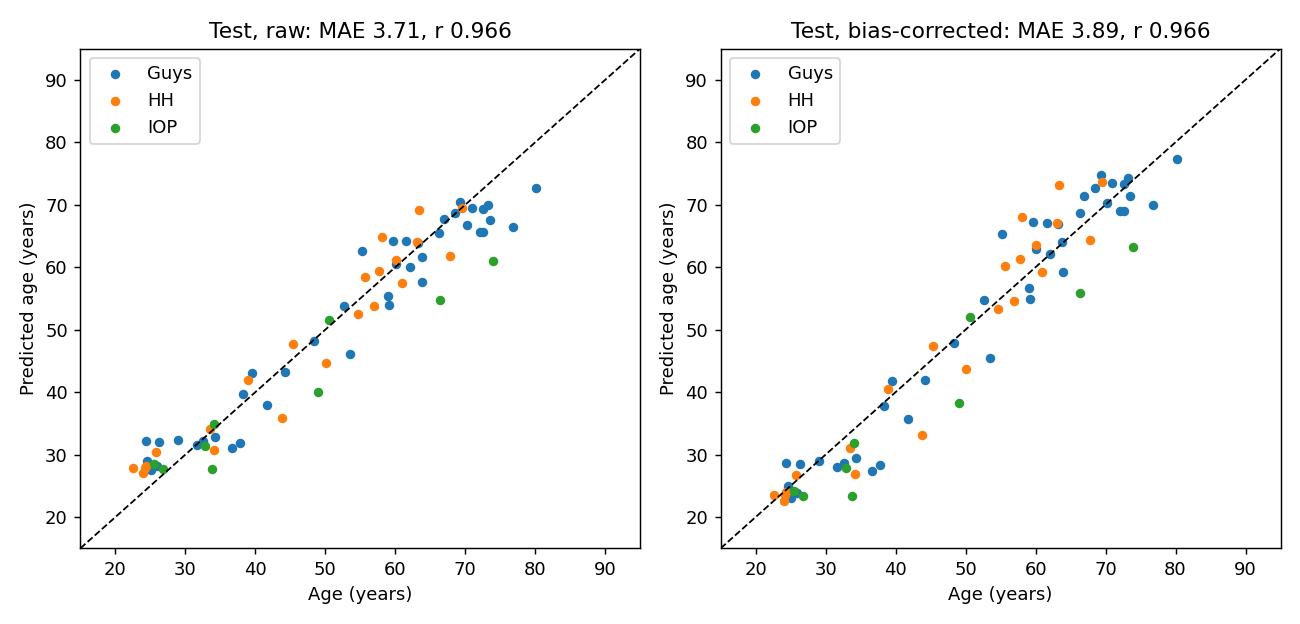
\includegraphics[width=\columnwidth]{test_scatter.png}
\caption{Fine-tuned SFCN on the test set, raw (left) and bias-corrected (right), coloured by acquisition site.}
\label{fig:scatter}
\end{figure}

\subsection{Group fairness: sex and acquisition site}
Table~\ref{tab:fair} and Fig.~\ref{fig:fair} show the age-adjusted test-set differences. There is \textbf{no detectable sex difference} in BAG or error, with intervals narrow enough to exclude differences larger than about 2--3 years. In contrast, IOP scans receive a corrected BAG \textbf{5.06 years lower} than Guys scans ($p=0.012$); 8 of the 9 IOP test subjects have a negative gap, and leaving out each IOP subject in turn gives offsets between $-4.18$ and $-5.93$. No group difference in absolute error has a CI excluding zero.

The IOP offset is absent in the training subjects, which the model fits closely ($-0.97$ \ci{-3.09}{+1.15}), and appears independently in validation ($-4.08$ \ci{-7.31}{-0.85}) and test ($-5.06$): it is a failure to generalise to \emph{new} IOP individuals, not a chance finding in one split. LOSO confirms this: a model never trained on IOP is \textbf{3.30 years} \ci{1.62}{4.93} less accurate there (MAE 6.80 vs 3.59), whereas a model never trained on HH generalises (+0.25 \ci{-0.88}{1.36}).

\begin{table}[t]
\caption{Age-adjusted group differences, test set (95\% CI)}
\label{tab:fair}
\centering
\setlength{\tabcolsep}{4pt}
\begin{tabular}{lcc}
\toprule
Comparison & Corrected BAG (yrs) & $|$Error$|$ (yrs) \\
\midrule
Male vs female & $-0.59$ \ci{-2.67}{+1.64} & $-0.64$ \ci{-1.90}{+0.59} \\
HH vs Guys     & $+1.06$ \ci{-1.44}{+3.53} & $+0.19$ \ci{-1.07}{+1.47} \\
IOP vs Guys    & $\mathbf{-5.06}$ \ci{-8.66}{-1.34} & $+1.92$ \ci{-1.36}{+5.14} \\
\bottomrule
\end{tabular}
\end{table}

\begin{figure}[t]
\centering
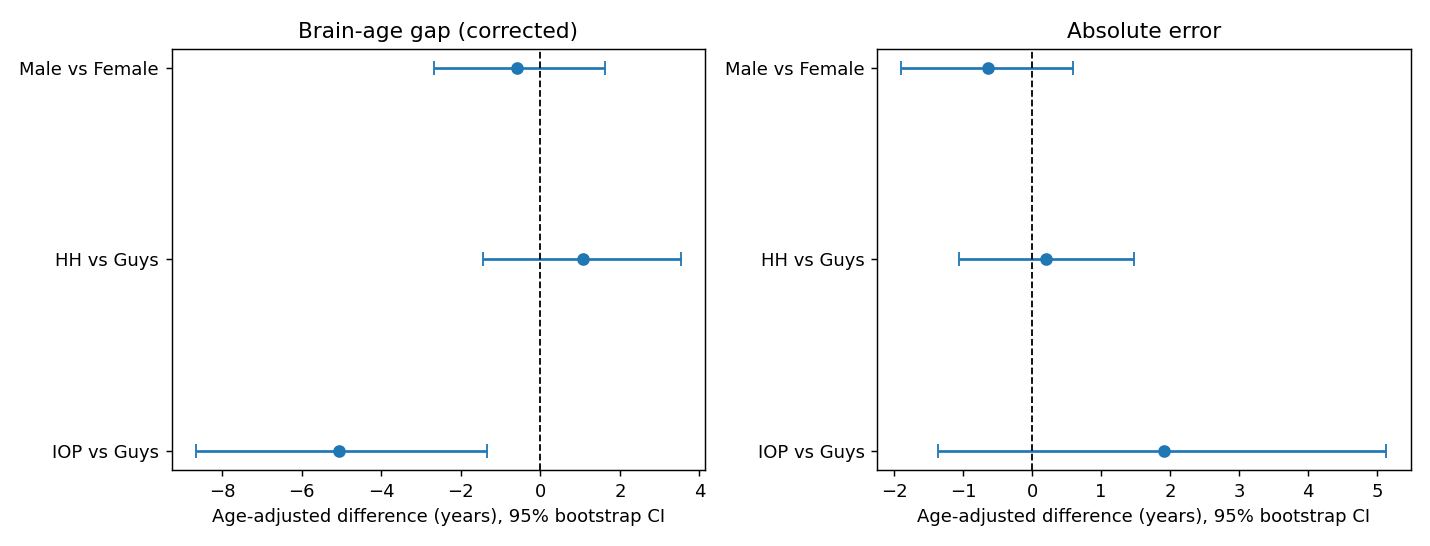
\includegraphics[width=\columnwidth]{fairness_effects.png}
\caption{Age-adjusted group differences in corrected BAG (left) and absolute error (right) on the test set, with 95\% bootstrap CIs.}
\label{fig:fair}
\end{figure}

\subsection{Where does the model look, and can we trust it?}
Attribution concentrates on the deep grey matter around the lateral ventricles (thalamus, caudate, putamen), the periventricular white matter and the cerebellum (Fig.~\ref{fig:attr}), structures known to change with age. Re-initialising the top layers changes the maps almost completely (median Spearman $\rho=0.13$), so the maps depend on what the model learned. In the deletion test (Table~\ref{tab:del}), removing the top-ranked 5\% of cells changes the prediction by 4.83 years, against 1.04 for random and 0.46 for bottom-ranked cells; top beats random by +3.79 years \ci{3.03}{4.66} in 93\% of subjects (Wilcoxon $p=5\times10^{-11}$), and the ordering holds at every fraction.

After FDR correction, no region differs by sex. Attribution patterns differ between acquisition sites: relative to Guys, HH and IOP place less attribution on deep grey matter ($-1.14$ and $-1.29$ percentage points) and more on the cerebellum and unlabelled tissue.

\begin{figure}[t]
\centering
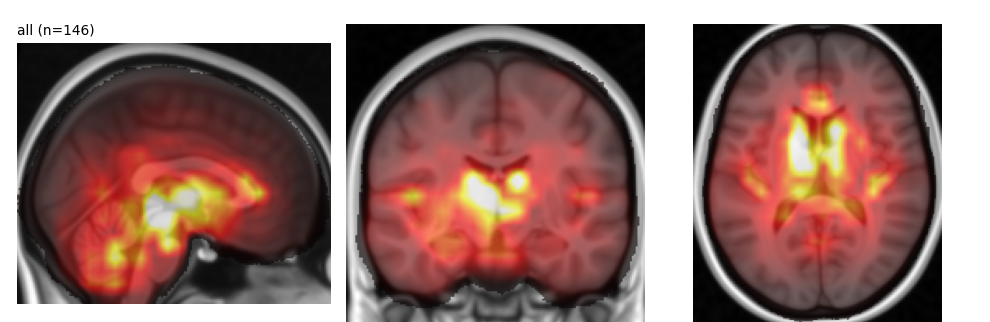
\includegraphics[width=\columnwidth]{attribution_mean_map.png}\\[2pt]
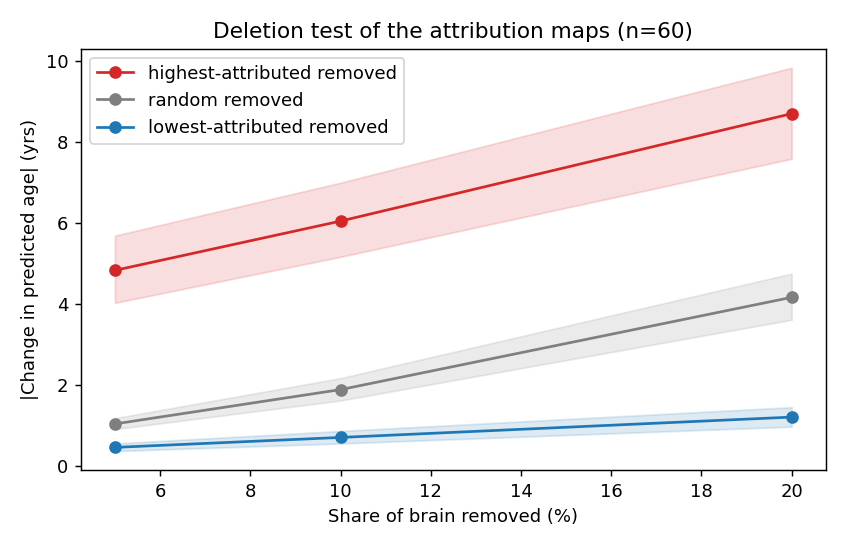
\includegraphics[width=0.82\columnwidth]{deletion_test.png}
\caption{Top: mean attribution map over held-out subjects. Bottom: deletion test, $|\Delta$ predicted age$|$ when top-, randomly- or bottom-ranked regions are smoothed away.}
\label{fig:attr}
\end{figure}

\begin{table}[t]
\caption{Deletion test: $|\Delta$ predicted age$|$ (years), 60 subjects}
\label{tab:del}
\centering
\begin{tabular}{lccc}
\toprule
Fraction removed & Top-ranked & Random & Bottom-ranked \\
\midrule
5\%  & \textbf{4.83} & 1.04 & 0.46 \\
10\% & \textbf{6.05} & 1.89 & 0.70 \\
20\% & \textbf{8.71} & 4.17 & 1.21 \\
\bottomrule
\end{tabular}
\end{table}

\subsection{Is the model right for the wrong reasons?}
\textbf{The representation encodes the acquisition site.} A linear probe on the 64-d features identifies the site of held-out scans with 93.5\% balanced accuracy, and \textbf{91.2\%} \ci{86.6}{95.2} after age and sex are regressed out, against 40.8\% from demographics alone (Table~\ref{tab:probe}, Fig.~\ref{fig:probe}). All 18 held-out IOP scans were identified and no other scan was labelled IOP. The signature is already present in the pretrained network (92.8\%), so it reflects image appearance that survives preprocessing rather than something learned from IXI. This shows that site information is \emph{present}; the next test asks whether the prediction \emph{responds} to it.

\begin{table}[t]
\caption{Site probe on held-out subjects (chance 33\%)}
\label{tab:probe}
\centering
\begin{tabular}{lc}
\toprule
Features & Balanced accuracy (\%) \\
\midrule
Age and sex only & 40.8 \ci{31.2}{50.9} \\
Input intensity quantiles & 99.6 \ci{98.7}{100} \\
Pretrained SFCN (never saw IXI) & 92.8 \ci{87.2}{96.9} \\
Fine-tuned SFCN & 93.5 \ci{88.1}{97.7} \\
Fine-tuned SFCN, age/sex removed & \textbf{91.2} \ci{86.6}{95.2} \\
After ComBat harmonisation & 36.3 \\
\bottomrule
\end{tabular}
\end{table}

\begin{figure}[t]
\centering
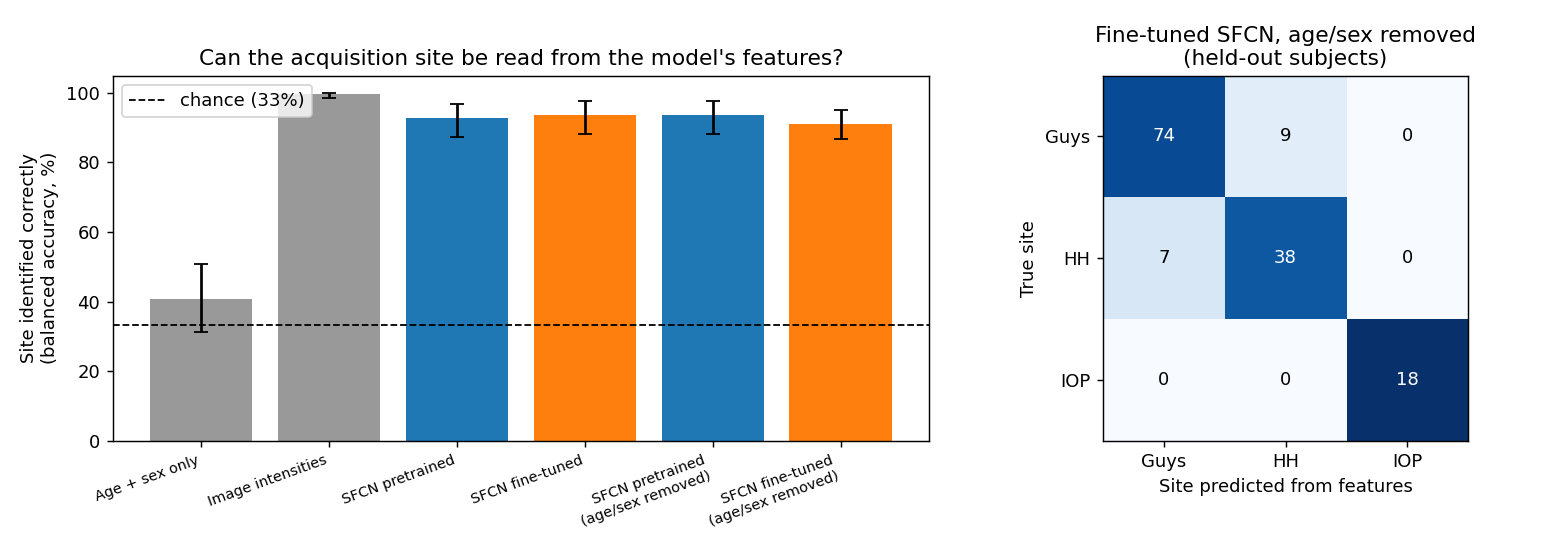
\includegraphics[width=\columnwidth]{site_probe.png}
\caption{Site probe: balanced accuracy by feature set (left) and confusion matrix for fine-tuned features with age and sex removed (right).}
\label{fig:probe}
\end{figure}

\textbf{Predicted age responds to acquisition appearance.} Changing only the intensity appearance of the same brains shifts predicted age substantially (Fig.~\ref{fig:stress}). Relative to the own-site match, HH brains given an IOP appearance became \textbf{3.92 years younger} \ci{-4.47}{-3.38} (45 of 45 subjects), and IOP brains given an HH appearance became \textbf{3.14 years older} \ci{2.44}{3.97} (18 of 18). Among single properties, strong blur ($\sigma=1.5$ voxels) lowered predicted age by 3.17 years \ci{1.24}{5.11}, contrast changes moved it by 0.4--0.9 years and noise and non-uniformity by less. The same anatomy therefore receives a different age depending on acquisition appearance.

\begin{figure*}[t]
\centering
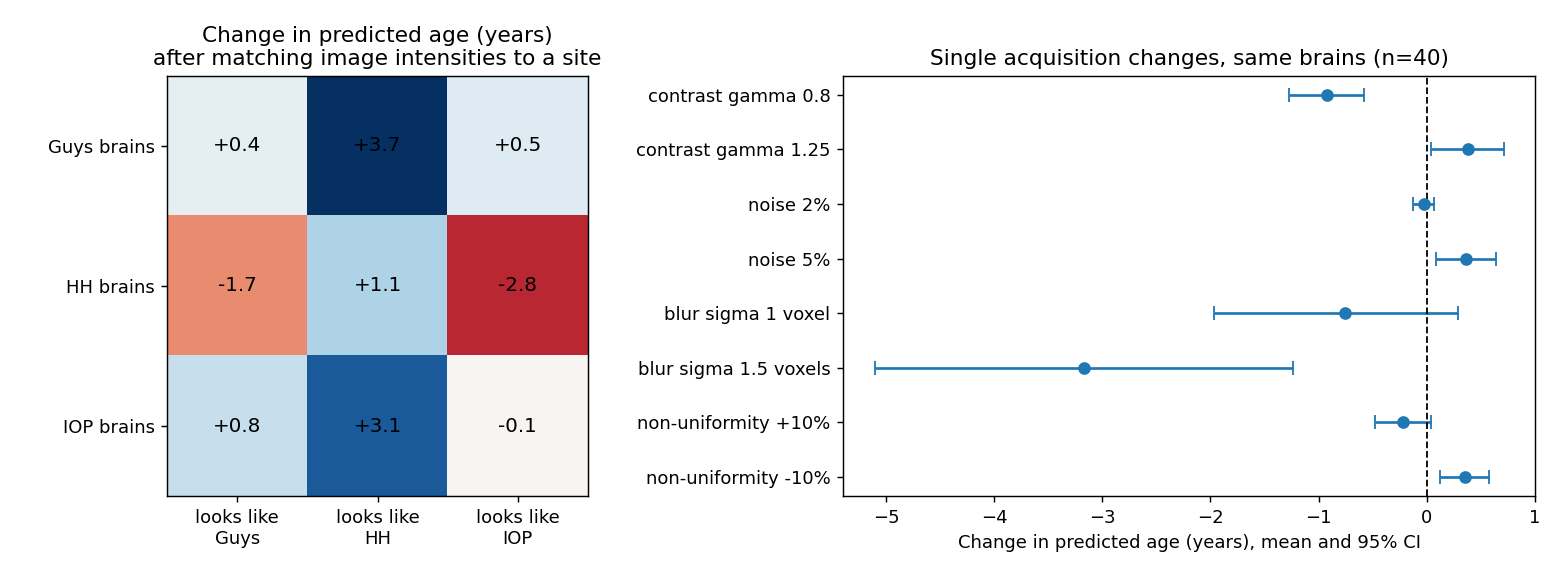
\includegraphics[width=0.85\textwidth]{stress_test.png}
\caption{Acquisition stress test. Left: change in predicted age when each site's held-out brains are given each site's age- and sex-standardised intensity appearance (relative to own-site matching). Right: single acquisition perturbations.}
\label{fig:stress}
\end{figure*}

\textbf{What the IOP offset is not.} We tested three acquisition explanations at IOP's measured levels (Table~\ref{tab:ruleout}). (i) \emph{Global intensity:} after age/sex standardisation, swapping between the Guys and IOP appearances moved predicted age by at most about 1 year; without standardisation the effect looked larger ($-0.60/+1.60$) because IOP's younger recruitment had leaked into its reference. (ii) \emph{Smoothness:} native resolution is identical across sites ($0.94\times0.94\times1.2$\,mm), yet IOP inputs are markedly smoother (FWHM +0.87\,mm, +2.38 SD vs Guys, age/sex-adjusted). Blurring Guys and HH brains to IOP's smoothness did \emph{not} lower predicted age. (iii) \emph{Site signature:} ComBat removed the representation's site signature (probe $91.2\rightarrow36.3\%$) at no cost in accuracy (held-out MAE $3.81\rightarrow3.90$), but the IOP offset largely persisted, $-4.53\rightarrow-3.95$ years (Fig.~\ref{fig:combat}).

\begin{table}[t]
\caption{Rule-out tests for the IOP offset (years, 95\% CI)}
\label{tab:ruleout}
\centering
\setlength{\tabcolsep}{3pt}
\begin{tabular}{lc}
\toprule
Test at IOP's measured level & Effect \\
\midrule
Guys $\rightarrow$ IOP intensity look & $+0.11$ \ci{-0.18}{+0.39} \\
IOP $\rightarrow$ Guys intensity look & $+0.90$ \ci{+0.17}{+1.70} \\
Guys blurred to IOP smoothness & $+0.93$ \ci{+0.60}{+1.28} \\
HH blurred to IOP smoothness & $+0.01$ \ci{-0.32}{+0.36} \\
IOP offset before ComBat & $-4.53$ \ci{-7.04}{-2.01} \\
IOP offset after ComBat & $-3.95$ \ci{-6.40}{-1.37} \\
\bottomrule
\multicolumn{2}{l}{\footnotesize None reproduces a 5-year younger prediction.}
\end{tabular}
\end{table}

\begin{figure*}[t]
\centering
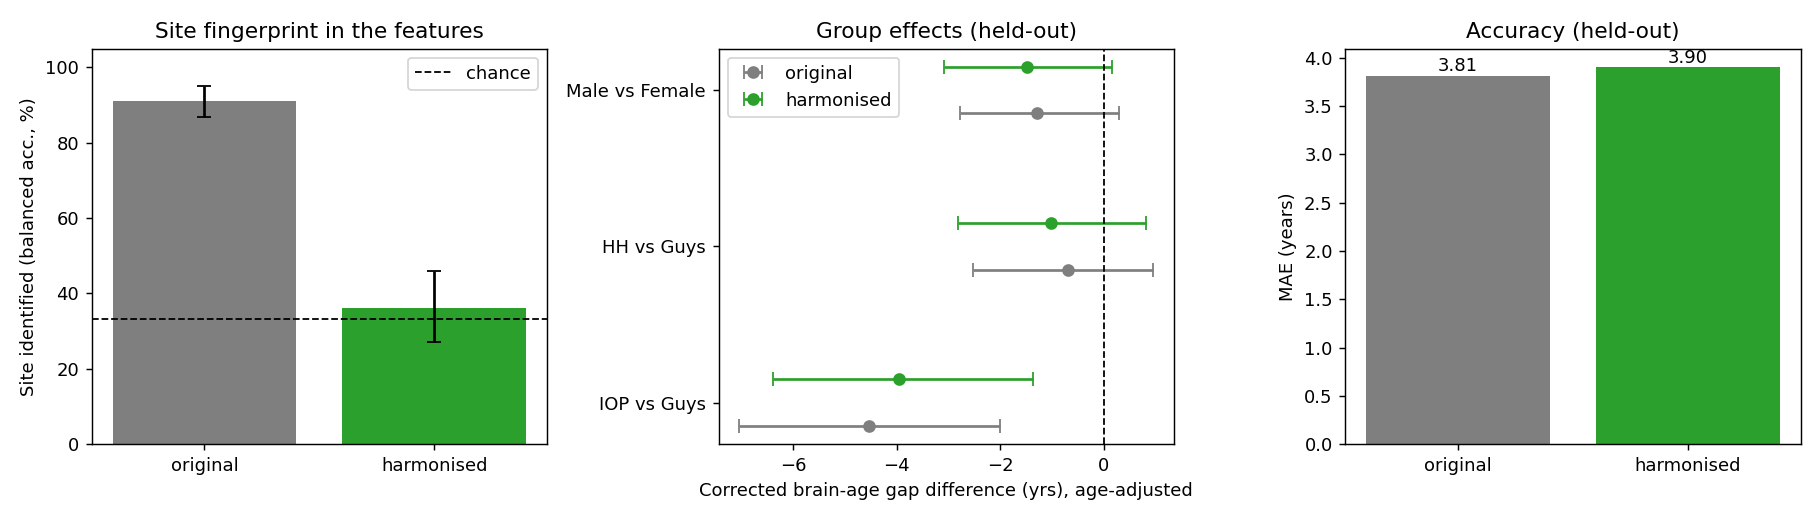
\includegraphics[width=0.95\textwidth]{harmonisation.png}
\caption{ComBat feature harmonisation: the site fingerprint is removed (left), accuracy is unchanged (right), but most of the IOP offset remains (middle).}
\label{fig:combat}
\end{figure*}

\subsection{Does the model know when it is unsure?}
The model's predictive spread was larger for IOP (8.06 years vs 5.66 Guys and 6.39 HH; adjusted +2.48 \ci{1.30}{3.65}), and its 90\% ranges contained the true age for 88\% of held-out subjects. The model never trained on IOP was twice as uncertain there (12.46 vs 6.13; +5.32 \ci{4.65}{5.99}) yet kept 92\% coverage despite an MAE of 6.80: it is less accurate but signals it, rather than being confidently wrong (Fig.~\ref{fig:unc}). For HH, which LOSO generalises to, uncertainty barely rose (+0.79). Per subject, uncertainty tracked error only weakly (Spearman 0.16), so it is a group-level warning, not a per-scan error detector.

\begin{figure*}[t]
\centering
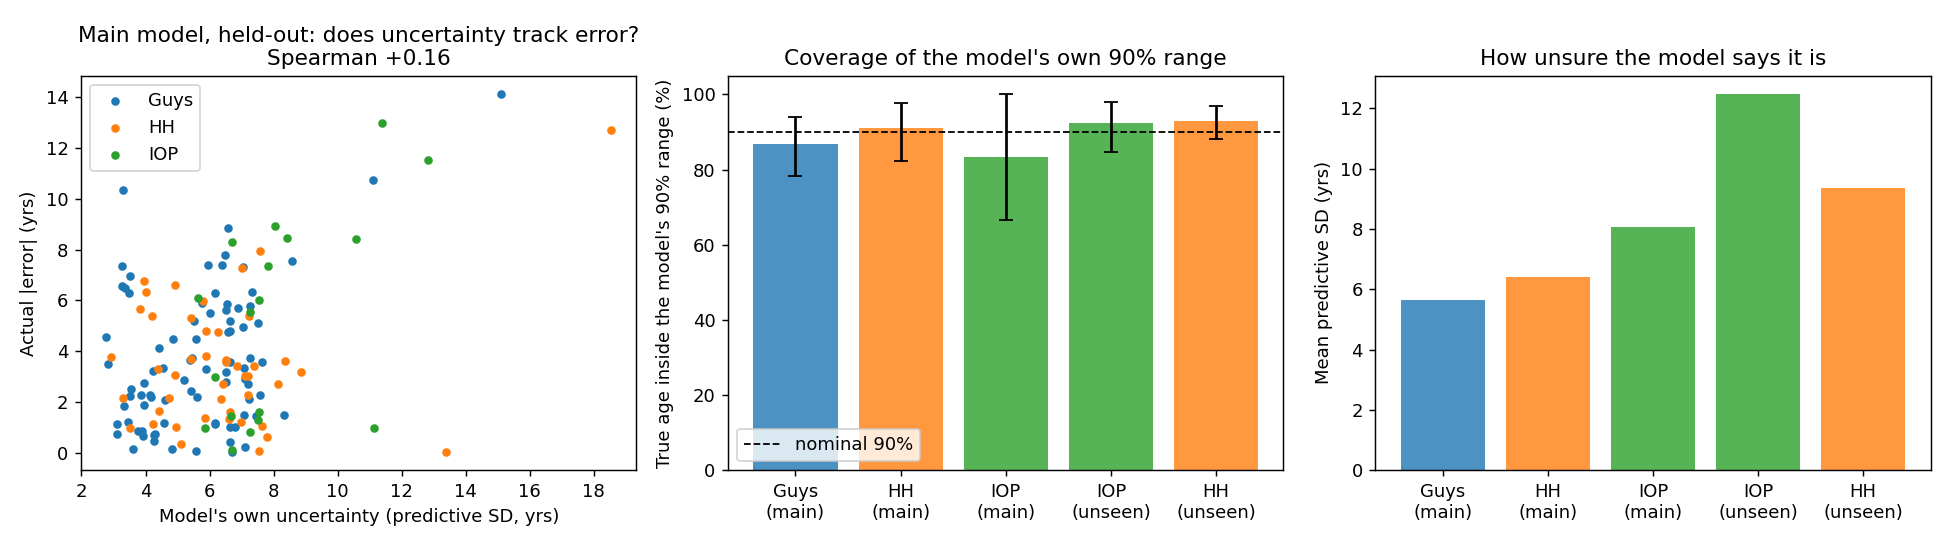
\includegraphics[width=0.95\textwidth]{uncertainty.png}
\caption{Predictive uncertainty. Left: uncertainty against absolute error. Middle: coverage of the model's own 90\% range. Right: mean uncertainty by site for the main model and the leave-one-site-out models.}
\label{fig:unc}
\end{figure*}

\subsection{Model fairness passport}
Table~\ref{tab:passport} condenses the audit into six verdicts. The full one-page passport, with evidence and usage guidance (suitable for single-site research; not for clinical use or uncorrected cross-scanner comparison), is released with the code.

\begin{table}[t]
\caption{Model fairness passport: summary verdicts}
\label{tab:passport}
\centering
\setlength{\tabcolsep}{3pt}
\begin{tabular}{llp{3.6cm}}
\toprule
Check & Verdict & Evidence \\
\midrule
Accuracy & \textcolor{green!45!black}{\textbf{PASS}} & MAE 3.71, $r$ 0.966 \\
Fair by sex & \textcolor{green!45!black}{\textbf{PASS}} & $-0.59$ yrs, CI spans 0 \\
Fair by site & \textcolor{red!70!black}{\textbf{FAIL}} & IOP $-5.06$ yrs, replicated \\
Scanner invariance & \textcolor{red!70!black}{\textbf{FAIL}} & site probe 91\%; look shifts 3--4 yrs \\
Faithful explanations & \textcolor{green!45!black}{\textbf{PASS}} & $\rho$ 0.13; deletion 4.83 vs 1.04 \\
Honest uncertainty & \textcolor{green!45!black}{\textbf{PASS}} & doubles when unseen; 92\% coverage \\
\bottomrule
\end{tabular}
\end{table}

%=====================================================================
\section{Discussion}
%=====================================================================
\textbf{Accurate and fair across sex.} The fine-tuned SFCN predicts age on IXI with an error under 4 years, and we found no sex difference in BAG, error or attribution.

\textbf{A robust acquisition-site effect.} IOP stands out in every analysis: its BAG is about 5 years lower in two independent splits, it is the only site a model cannot generalise to unseen, it is the most distinct site in the representation, and the model is most uncertain about it. These are acquisition-site effects in the descriptive sense; because site is confounded with each site's recruited population in IXI, this design cannot attribute them to the scanner rather than the cohort.

\textbf{Partly right for the wrong reasons.} The representation identifies the site at 91\% accuracy even after removing age and sex and before fine-tuning, and the prediction moves by 3--4 years when only a scan's intensity appearance changes. The model is therefore not acquisition-invariant: an unchanged brain could receive a different brain age on a different scanner, which matters for any comparison of BAG across sites.

\textbf{But the IOP offset is not a simple scanner artefact.} The obvious acquisition explanations fail at IOP's measured levels: the global intensity profile accounts for about 1 year, matched smoothness for none, and removing the site signature leaves most of the offset. Combined with the offset appearing only for new IOP individuals, this points either to acquisition properties not modelled here (e.g., the spatial pattern of tissue contrast or vendor-specific reconstruction) or to genuine cohort differences. Two methodological lessons follow: an intensity reference that is not standardised for recruitment age overstated the intensity effect, and a harmonisation method that erases a site signature need not remove a site disparity. Reporting a site disparity as ``scanner bias'' without such tests would have been wrong here.

\textbf{The model flags the problem itself.} Elevated group-level uncertainty on a new site, with near-nominal coverage, could serve as a warning that BAGs there should not be compared directly with other sites.

\textbf{Limitations.} Subgroups are small (9 IOP test and 18 held-out subjects), although the offset replicated across splits. We used a single seed and split, so CIs reflect subject sampling, not training randomness. Site is confounded with cohort in IXI. Quantile matching changes only the global intensity distribution, and Gaussian blur did not reproduce IOP's full sharpness profile. ComBat was applied to pooled features without retraining the head; image-level harmonisation or adversarial training \cite{dinsdale2021unlearning} may behave differently. The attribution resolution is 8\,mm, and deletion tests are themselves affected by distribution shift. The uncertainty is the softmax spread of a soft-label model, not a calibrated interval \cite{guo2017calibration}. Participants are healthy volunteers, and no clinical conclusion follows.

\textbf{Future work.} Travelling-subject data (the same people scanned at several sites) would separate scanner from cohort; further directions are site-adversarial fine-tuning, multiple seeds and splits, and extending the passport to other datasets and models.

%=====================================================================
\section{Conclusion}
%=====================================================================
A fine-tuned SFCN brain-age model is accurate on IXI and shows no sex disparity, but it is not acquisition-invariant: it carries a strong site signature, its predictions shift with acquisition appearance alone, and one site shows a robust 5-year offset and poor generalisation when unseen. That offset is not explained by intensity, smoothness or the representation's site signature, and its cause cannot be determined from IXI. Its explanations are faithful and its uncertainty rises where it is least reliable. Auditing beyond accuracy changed the answer to ``is this model good?'': it is accurate, but its brain-age gaps should not be compared across acquisition sites without site-aware validation.

\section*{Code and Data Availability}
All code, including preprocessing, training, every analysis, an interactive results website, a live browser demo and the fairness passport, is available at \url{https://github.com/Jaaiwanth/brain-age-fairness-xai}. IXI is publicly available under CC BY-SA 3.0 \cite{ixi}.

\section*{Author Contributions}
Adharshan N and Jaaiwanth K contributed equally. Both authors jointly designed the study, built and verified the corrected labels, developed the preprocessing and fine-tuning pipelines (including the independent SFCN and DeepBrainNet replication), performed the fairness, attribution, shortcut and uncertainty analyses, built the website, demo and passport, and wrote the manuscript. Shridevi S supervised the project and reviewed the manuscript.

\section*{Acknowledgment}
We thank the IXI project for making the data publicly available, and the authors of SFCN for releasing their pretrained weights.

\bibliographystyle{IEEEtran}
\bibliography{refs}

\end{document}
